% Options for packages loaded elsewhere
\PassOptionsToPackage{unicode}{hyperref}
\PassOptionsToPackage{hyphens}{url}
\PassOptionsToPackage{dvipsnames,svgnames,x11names}{xcolor}
%
\documentclass[
]{estat/estat}

\usepackage{amsmath,amssymb}
\usepackage{iftex}
\ifPDFTeX
  \usepackage[T1]{fontenc}
  \usepackage[utf8]{inputenc}
  \usepackage{textcomp} % provide euro and other symbols
\else % if luatex or xetex
  \usepackage{unicode-math}
  \defaultfontfeatures{Scale=MatchLowercase}
  \defaultfontfeatures[\rmfamily]{Ligatures=TeX,Scale=1}
\fi
\usepackage{lmodern}
\ifPDFTeX\else  
    % xetex/luatex font selection
    \setmainfont[]{Arial}
\fi
% Use upquote if available, for straight quotes in verbatim environments
\IfFileExists{upquote.sty}{\usepackage{upquote}}{}
\IfFileExists{microtype.sty}{% use microtype if available
  \usepackage[]{microtype}
  \UseMicrotypeSet[protrusion]{basicmath} % disable protrusion for tt fonts
}{}
\makeatletter
\@ifundefined{KOMAClassName}{% if non-KOMA class
  \IfFileExists{parskip.sty}{%
    \usepackage{parskip}
  }{% else
    \setlength{\parindent}{0pt}
    \setlength{\parskip}{6pt plus 2pt minus 1pt}}
}{% if KOMA class
  \KOMAoptions{parskip=half}}
\makeatother
\usepackage{xcolor}
\usepackage[left=3cm,right=2cm,top=3cm,bottom=2cm]{geometry}
\setlength{\emergencystretch}{3em} % prevent overfull lines
\setcounter{secnumdepth}{5}
% Make \paragraph and \subparagraph free-standing
\makeatletter
\ifx\paragraph\undefined\else
  \let\oldparagraph\paragraph
  \renewcommand{\paragraph}{
    \@ifstar
      \xxxParagraphStar
      \xxxParagraphNoStar
  }
  \newcommand{\xxxParagraphStar}[1]{\oldparagraph*{#1}\mbox{}}
  \newcommand{\xxxParagraphNoStar}[1]{\oldparagraph{#1}\mbox{}}
\fi
\ifx\subparagraph\undefined\else
  \let\oldsubparagraph\subparagraph
  \renewcommand{\subparagraph}{
    \@ifstar
      \xxxSubParagraphStar
      \xxxSubParagraphNoStar
  }
  \newcommand{\xxxSubParagraphStar}[1]{\oldsubparagraph*{#1}\mbox{}}
  \newcommand{\xxxSubParagraphNoStar}[1]{\oldsubparagraph{#1}\mbox{}}
\fi
\makeatother


\providecommand{\tightlist}{%
  \setlength{\itemsep}{0pt}\setlength{\parskip}{0pt}}\usepackage{longtable,booktabs,array}
\usepackage{calc} % for calculating minipage widths
% Correct order of tables after \paragraph or \subparagraph
\usepackage{etoolbox}
\makeatletter
\patchcmd\longtable{\par}{\if@noskipsec\mbox{}\fi\par}{}{}
\makeatother
% Allow footnotes in longtable head/foot
\IfFileExists{footnotehyper.sty}{\usepackage{footnotehyper}}{\usepackage{footnote}}
\makesavenoteenv{longtable}
\usepackage{graphicx}
\makeatletter
\def\maxwidth{\ifdim\Gin@nat@width>\linewidth\linewidth\else\Gin@nat@width\fi}
\def\maxheight{\ifdim\Gin@nat@height>\textheight\textheight\else\Gin@nat@height\fi}
\makeatother
% Scale images if necessary, so that they will not overflow the page
% margins by default, and it is still possible to overwrite the defaults
% using explicit options in \includegraphics[width, height, ...]{}
\setkeys{Gin}{width=\maxwidth,height=\maxheight,keepaspectratio}
% Set default figure placement to htbp
\makeatletter
\def\fps@figure{htbp}
\makeatother

\authors{%
    Bruno Boaventura Xavier\\

    
}

% escreva o nome do cliente aqui
% se for mais de um separe por \\
\client{%
    House of Excellence
}
% Baixando pacotes
\RequirePackage{fancyhdr}
\RequirePackage{graphicx}

\setlength\headheight{28pt}  

\setlength{\parindent}{15pt} % Adiciona indentação nos parágrafos
\setlength{\parskip}{0pt} % Adiciona 0 espaço entro os parágrafos

\newcommand{\estat}{\textbf{ESTAT}\xspace}
\newcommand{\direx}{\textbf{DIREX}\xspace}
\makeatletter
\@ifpackageloaded{caption}{}{\usepackage{caption}}
\AtBeginDocument{%
\ifdefined\contentsname
  \renewcommand*\contentsname{Índice}
\else
  \newcommand\contentsname{Índice}
\fi
\ifdefined\listfigurename
  \renewcommand*\listfigurename{Lista de Figuras}
\else
  \newcommand\listfigurename{Lista de Figuras}
\fi
\ifdefined\listtablename
  \renewcommand*\listtablename{Lista de Tabelas}
\else
  \newcommand\listtablename{Lista de Tabelas}
\fi
\ifdefined\figurename
  \renewcommand*\figurename{Figura}
\else
  \newcommand\figurename{Figura}
\fi
\ifdefined\tablename
  \renewcommand*\tablename{Tabela}
\else
  \newcommand\tablename{Tabela}
\fi
}
\@ifpackageloaded{float}{}{\usepackage{float}}
\floatstyle{ruled}
\@ifundefined{c@chapter}{\newfloat{codelisting}{h}{lop}}{\newfloat{codelisting}{h}{lop}[chapter]}
\floatname{codelisting}{Listagem}
\newcommand*\listoflistings{\listof{codelisting}{Lista de Listagens}}
\captionsetup{labelsep=colon}
\makeatother
\makeatletter
\makeatother
\makeatletter
\@ifpackageloaded{caption}{}{\usepackage{caption}}
\@ifpackageloaded{subcaption}{}{\usepackage{subcaption}}
\makeatother

\ifLuaTeX
\usepackage[bidi=basic]{babel}
\else
\usepackage[bidi=default]{babel}
\fi
\babelprovide[main,import]{portuguese}
\ifPDFTeX
\else
\babelfont{rm}[]{Arial}
\fi
% get rid of language-specific shorthands (see #6817):
\let\LanguageShortHands\languageshorthands
\def\languageshorthands#1{}
\ifLuaTeX
  \usepackage{selnolig}  % disable illegal ligatures
\fi
\usepackage{bookmark}

\IfFileExists{xurl.sty}{\usepackage{xurl}}{} % add URL line breaks if available
\urlstyle{same} % disable monospaced font for URLs
\hypersetup{
  pdftitle={Projeto Fantasma},
  pdflang={pt},
  colorlinks=true,
  linkcolor={black},
  filecolor={black},
  citecolor={black},
  urlcolor={black},
  pdfcreator={LaTeX via pandoc}}


\title{Projeto Fantasma}
\author{}
\date{}

\begin{document}
\maketitle

% Limpando tudo
\fancyhf{} 

% Ajustes do header
\fancyhead[L]{} % limpando o lado esquerdo
\fancyhead[R]{
\includegraphics[width=0.20\textwidth]{estat/imagens/estat.png}} % adicionando logo no canto direito
\renewcommand{\headrulewidth}{0pt}   % sem linha embaixo da logo

% Ajustes de fim de página
\fancyfoot[R]{\textcolor{white}{\thepage}} % Número em branco no canto direito

% Aplicando o estilo que acabamos de criar
\pagestyle{fancy} 

\renewcommand*\contentsname{Sumário}
{
\hypersetup{linkcolor=}
\setcounter{tocdepth}{3}
\tableofcontents
}

\subsection{IMC por Esporte}\label{imc-por-esporte}

Diante do banco de dados, obteve-se acesso às variáveis quantitativas
contínuas que descrevem o peso dos atletas em libras (lbs) e suas
respectivas alturas em metros (m), tendo isso o Índice de Massa Corporal
(IMC) de cada um dos atletas foi calculando, atribuindo uma nova
variável ao banco que também é classificada como quantitativa contínua,
para, assim, realizar as análises, além disso, durante os cálculos 14
atletas não tiveram ou suas alturas ou seus pesos computados no banco de
dados e por isso foram retirados da variável que contabiliza todos os
IMC's. Ainda, vale ressaltar que pelo interesse de observar como os
valores de IMC se distribuem, agrupou-se os dados em relação aos
Esportes de interesse, que são identificados como variável qualitativa
nominal, a qual não tem distinção de ordem dentro da categoria, além
disso, tanto homens, quanto mulheres foram agrupados igualmente,
conforme suas categorias olímpicas - Atletismo, Badminton, Ginástica,
Judô.

\begin{figure}

\caption{\label{fig-e-box-expli}Boxplot explicativo sobre seus
elementos}

\centering{

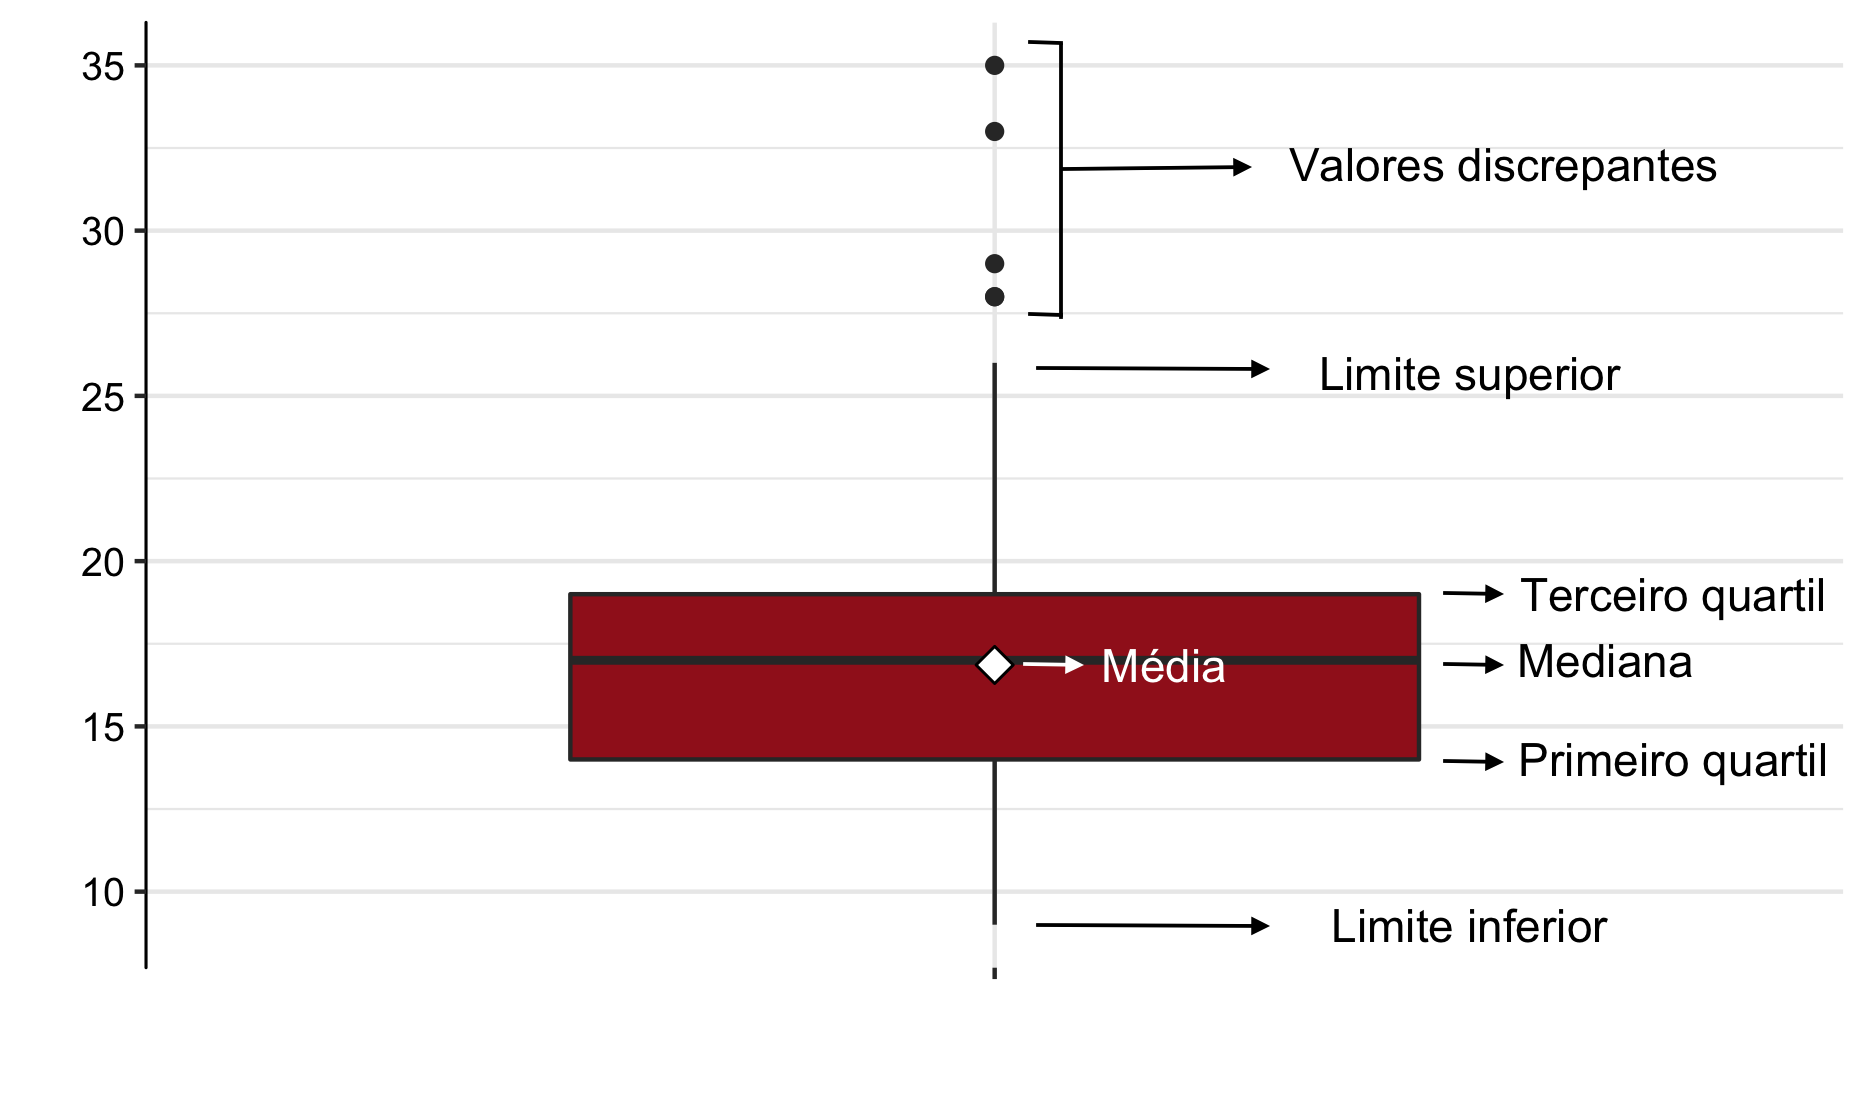
\includegraphics[width=158mm,height=\textheight]{images/box_uni.png}

}

\end{figure}%

Para analisar os dados obtidos serão utilizados \emph{boxplots} como
forma de visualização das informações e por meio da
\ref{fig-e-box-expli} apresenta-se o padrão e estruturação deles.

\begin{figure}[H]

\caption{\label{fig-boxplot}Boxplot do IMC pelos esportes}

\centering{

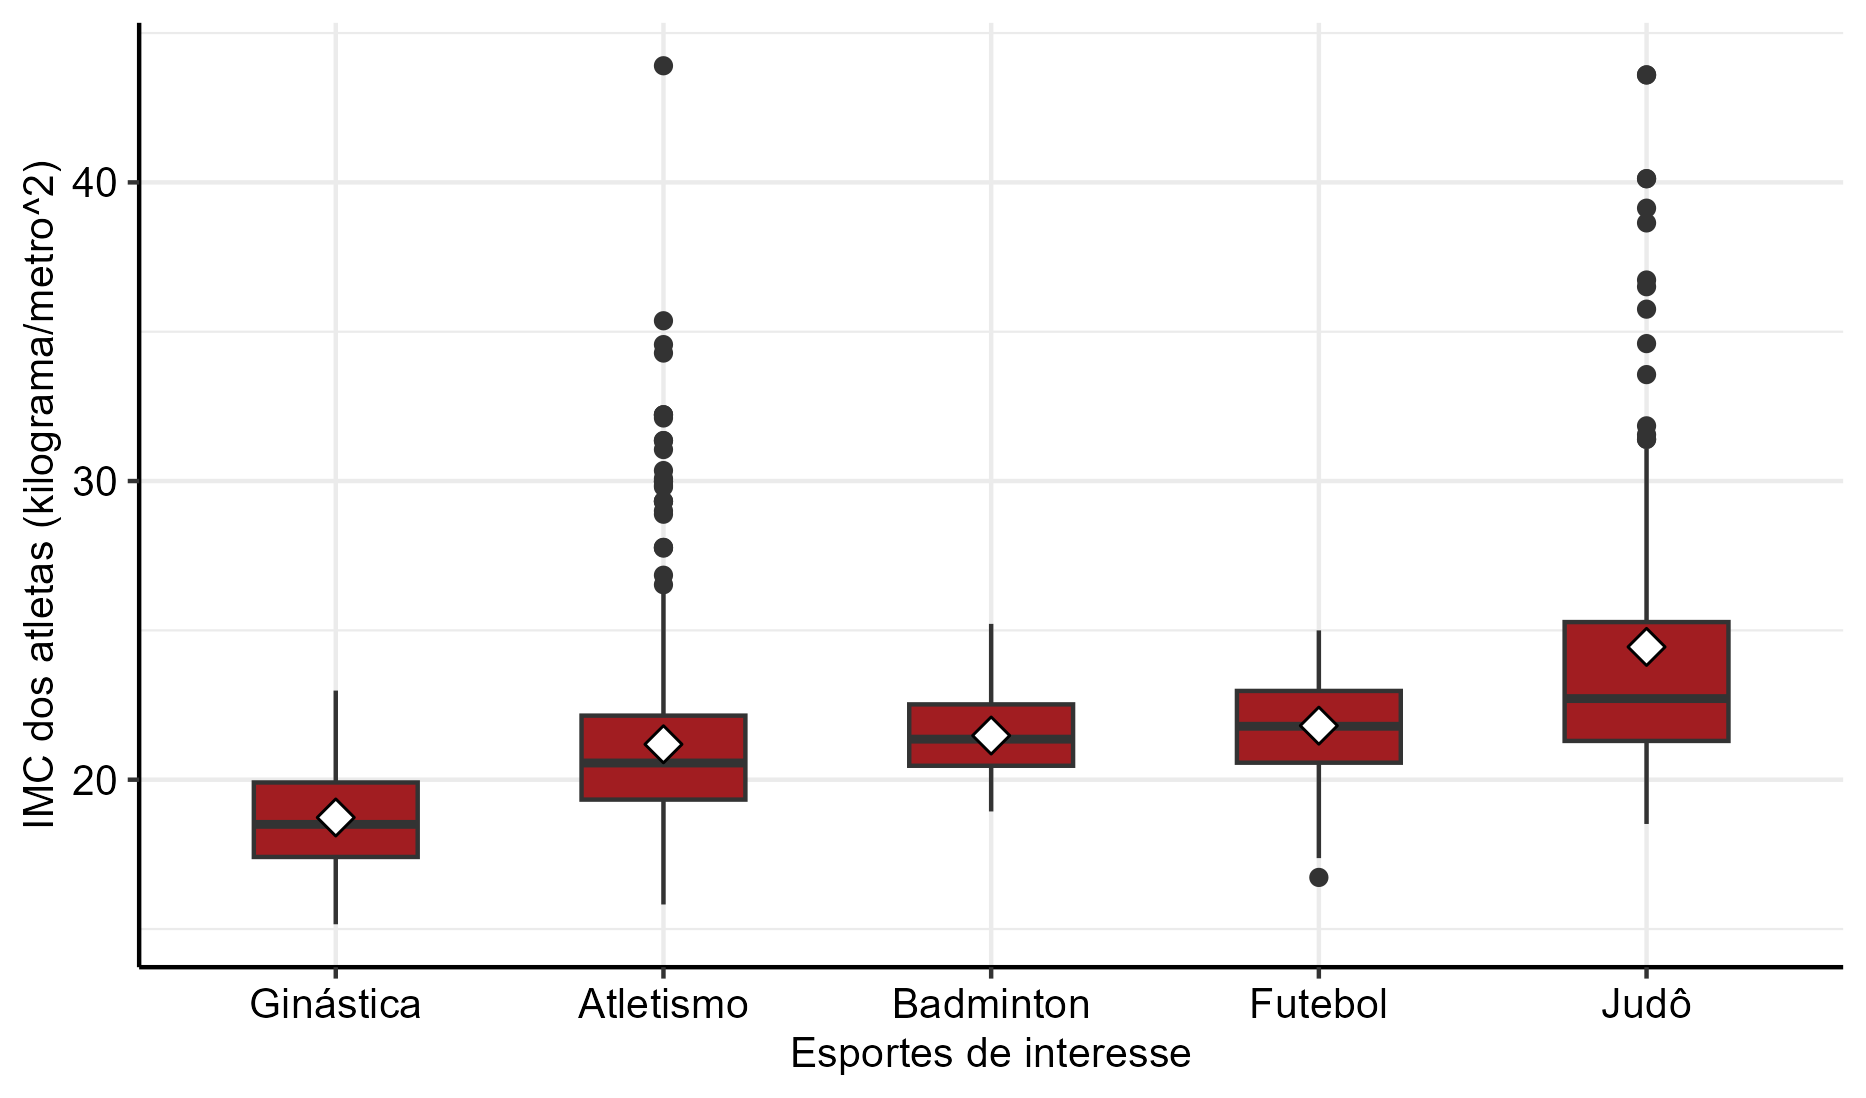
\includegraphics[width=158mm,height=\textheight]{images/box_bi.png}

}

\end{figure}%

\begin{table}[H]

\caption{\label{tbl-medidas}Medidas resumo do IMC por esportes}

\centering{

\begin{tabular}{ | l |         S[table-format = 2.2]         S[table-format = 1.2]         S[table-format = 2.2]         S[table-format = 2.2]         S[table-format = 2.2]         |} \toprule     \textbf{Estatística} & \textbf{Atletismo} & \textbf{Badminton} & \textbf{Futebol} & \textbf{Ginástica} & \textbf{Judô} \\     \midrule     Média & 22.30 & 22.21 & 22.51 & 20.68 & 25.70 \\     Desvio Padrão & 3.86 & 1.50 & 1.73 & 2.38 & 5.12 \\     Variância & 14.92 &  2.26 &  2.99 &  5.67 & 26.23 \\     Mínimo & 15.82 & 18.94 & 16.73 & 15.16 & 18.52 \\     1º Quartil & 20.03 & 21.22 & 21.34 & 18.61 & 22.06 \\     Mediana & 21.45 & 22.28 & 22.49 & 21.09 & 24.68 \\     3º Quartil & 23.67 & 23.21 & 23.71 & 22.48 & 27.70 \\     Máximo & 44.38 & 26.73 & 29.07 & 26.45 & 56.50 \\ \bottomrule \end{tabular}

}

\end{table}%

A partir da \ref{tbl-medidas} e da \ref{fig-boxplot} pode-se observar
que o Judô possui maior média de IMC (25,70), isso significa 3,19 a mais
que o segundo colocado - Futebol (22,51) - e maior mediana (24,68) entre
os esportes, esta também é seguida pelo Futebol como segundo maior valor
de mediana entre a população com 22,49, e por outro lado, a Ginástica
tem a menor media (20,68), obtendo um valor mais baixo que quarto menor
IMC médio - Badminton (22,21) - por uma diferença de 1,53, e menor
mediana (21,09) dentre eles, com 0,36 a menos que o Atletismo (21,45).
Além disso, consegue-se perceber que o Badminton possui, dentre os
valores mínimos, o mais alto (18,94), 0,42 a frente do Judô (18,52), e a
Ginástica o mais baixo (15,16), 0,66 a menos que o Atletismo. Já no
quesito de maior valor obtido do índice de massa corporal entre os
atletas está no Judô (56,50), 12,12 a mais que o Atletismo, e a
Ginástica com o menor novamente (26,45), o que representa 0,28 a menos
que Badminton.

Outrossim, observando os valores de 1º Quartil, 3º Quartil, Mediana,
Variância e Desvio Padrão, nota-se que o Badminton e Futebol possuem
valores de IMC mais próximos de primeiro e de terceiro quartil,
evidenciando estarem mais próximos da média, uma vez que a amplitude
interquartílica representa 50\% do total de todas as observações para a
determinada classe. Ainda, percebe-se que para ambos os Esportes suas
medianas, no caso do Badminton (22,28) e do Futebol (22,49) são também
próximos da média, convergindo para o entendimento que há maior
concentração dos valores em torno do valor médio. Sob outra perspectiva,
o Judô é a modalidade que o valores estão mais dispersos na amostra, o
que pode ser percebido pelo maior desvio padrão entre as modalidades
(5,12), assim como a variância (26,23), bem como sua amplitude
interquartil ser a maior entre os demais.

\begin{table}[H]

\caption{\label{tbl-tex}Coeficiente de variação dos esportes de
interesse}

\centering{

\begin{tabular}{l|r}   \hline \multicolumn{1}{l|}{\textbf{Esportes}} & \multicolumn{1}{r}{\textbf{Coeficiente de Variação}} \\   \hline Atletismo & 17,32\% \\ Badminton & 6,77\% \\ Futebol & 7,68\% \\ Ginástica & 11,51\% \\ Judô & 19,93\% \\   \hline \end{tabular}

}

\end{table}%

Antes de analisar a \ref{tbl-tex}, é preciso observar que O coeficiente
de variação auxilia ao fornecer a dispersão dos dados em relação à média
de maneira mais clara, já que seus resultados representam
percentualmente o quanto as classes estão concentradas em torno do valor
médio. De uma maneira mais direta, quanto menor for o seu valor, mais
homogêneos serão os dados, nesse caso homogêneo significa que os valores
não assumem valores dispersos. Portanto, para metrificar o coeficiente
de variação, entende-se como baixo (apontando um conjunto de dados
homogêneo) quando for menor ou igual a 25\%.

Com a \ref{tbl-tex} podemos comprovar o que havia sido analisado
outrora, dentre os demais esportes o que apresenta menor valor para o
Coeficiente de Variação foi o Badminton (6,77\%), ou seja, os atletas
que praticaram essa modalidade durantes as olimpíadas tiveram os valores
de IMC mais homogêneos em relação à média, seguido do Futebol (7,68\%) -
0,91\% de separação entre os dois - com 11,51\% de coeficiente de
variação está a Ginástica que dista 3,83\% do Futebol e possui 5,81\% a
menos de coeficiente que o Atletismo (17,31\%), este se distancia do
Judô (19,93\%) por 2,61\%, evidenciando que o Judô é o que possui os
valores mais dispersos, entretanto ainda se enquadrando como homogêneo.




\end{document}
